\section{Dynamics}
In order to archive complete system dynamics of spacecraft with array of N - VSCMGs, physical properties such as inertia and angular momentum of a single control moment gyroscope is evaluated first and latter for arrangement of spacecraft with multpile VSCMG units . Body fixed frame $\displaystyle \mathcal{F}_{b}$with basis vector $\displaystyle \{\hat{b}_{1} ,\hat{b}_{2} ,\hat{b}_{3}\}$ attached to center of mass of continuum rigid body at distance $\displaystyle \vec{r}_{0}$ from $\displaystyle \mathcal{F}_{i}$ as shown in \autoref{fig:tikRigidBody}. Body is rotating at angular velocity $\displaystyle \vec{\omega } =[ \omega _{1} \ \omega _{2} \ \omega _{3}]^{T}$ as shown in fig. The angular momentum $\displaystyle \delta \vec{\mathbf{h}}$ of infinitesimally small mass $\displaystyle \delta m$ at position $\displaystyle \vec{r} =[ x_{1} \ y_{2} \ z_{3}]^{T}$ in body, moving at velocity $\displaystyle \mathbf{\vec{v}} =\vec{\mathbf{\omega }} \times \vec{r}$ is expressed as
\begin{equation*}
\delta \vec{\mathbf{h}} =\ \vec{r} \times \delta m\mathbf{\vec{v}}
\end{equation*}
\begin{figure}[!ht]
    \centering
    

\tikzset{every picture/.style={line width=0.75pt}} %set default line width to 0.75pt        

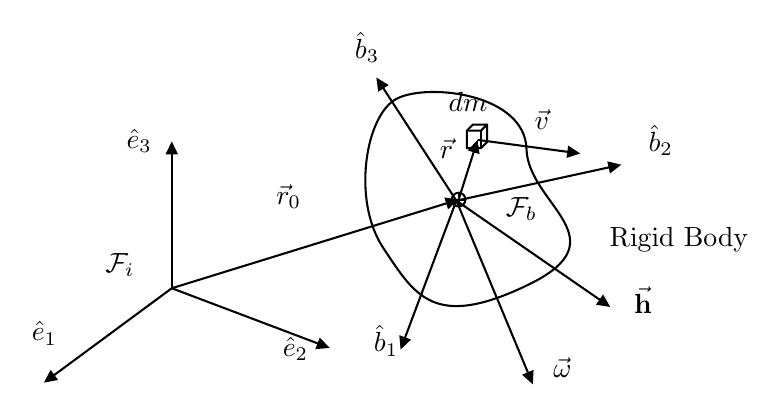
\begin{tikzpicture}[x=0.75pt,y=0.75pt,yscale=-1,xscale=1]
%uncomment if require: \path (0,197); %set diagram left start at 0, and has height of 197

%Straight Lines [id:da6848421575573145] 
\draw    (220.55,133.73) -- (161.35,177.43) ;
\draw [shift={(158.93,179.22)}, rotate = 323.56] [fill={rgb, 255:red, 0; green, 0; blue, 0 }  ][line width=0.08]  [draw opacity=0] (6.25,-3) -- (0,0) -- (6.25,3) -- cycle    ;
%Straight Lines [id:da9130919810329883] 
\draw    (220.55,133.73) -- (220.55,65.99) ;
\draw [shift={(220.55,62.99)}, rotate = 450] [fill={rgb, 255:red, 0; green, 0; blue, 0 }  ][line width=0.08]  [draw opacity=0] (6.25,-3) -- (0,0) -- (6.25,3) -- cycle    ;
%Straight Lines [id:da6717502672065161] 
\draw    (220.55,133.73) -- (293.81,161.42) ;
\draw [shift={(296.61,162.48)}, rotate = 200.71] [fill={rgb, 255:red, 0; green, 0; blue, 0 }  ][line width=0.08]  [draw opacity=0] (6.25,-3) -- (0,0) -- (6.25,3) -- cycle    ;
%Shape: Polygon Curved [id:ds602562353451706] 
\draw   (329.07,42.33) .. controls (344.28,34.72) and (390.68,40.05) .. (391.44,66.67) .. controls (392.2,93.29) and (437.84,110.03) .. (392.2,132.09) .. controls (346.56,154.15) and (337.59,137.03) .. (322.37,114.21) .. controls (307.16,91.39) and (313.85,49.94) .. (329.07,42.33) -- cycle ;
%Straight Lines [id:da39324245591715457] 
\draw    (357.65,91.54) -- (331.83,160.45) ;
\draw [shift={(330.78,163.26)}, rotate = 290.54] [fill={rgb, 255:red, 0; green, 0; blue, 0 }  ][line width=0.08]  [draw opacity=0] (6.25,-3) -- (0,0) -- (6.25,3) -- cycle    ;
%Straight Lines [id:da930908309847323] 
\draw    (357.65,91.54) -- (320.74,34.74) ;
\draw [shift={(319.1,32.22)}, rotate = 416.98] [fill={rgb, 255:red, 0; green, 0; blue, 0 }  ][line width=0.08]  [draw opacity=0] (6.25,-3) -- (0,0) -- (6.25,3) -- cycle    ;
%Straight Lines [id:da12681885554956018] 
\draw    (357.65,91.54) -- (434.17,74.84) ;
\draw [shift={(437.1,74.2)}, rotate = 527.69] [fill={rgb, 255:red, 0; green, 0; blue, 0 }  ][line width=0.08]  [draw opacity=0] (6.25,-3) -- (0,0) -- (6.25,3) -- cycle    ;
%Shape: Cube [id:dp2442226204871445] 
\draw   (362.69,57.8) -- (365.61,54.88) -- (372.43,54.88) -- (372.43,63.32) -- (369.5,66.24) -- (362.69,66.24) -- cycle ; \draw   (372.43,54.88) -- (369.5,57.8) -- (362.69,57.8) ; \draw   (369.5,57.8) -- (369.5,66.24) ;
%Straight Lines [id:da1664531723187539] 
\draw    (220.55,133.73) -- (355.87,91.9) ;
\draw [shift={(358.73,91.01)}, rotate = 522.8199999999999] [fill={rgb, 255:red, 0; green, 0; blue, 0 }  ][line width=0.08]  [draw opacity=0] (6.25,-3) -- (0,0) -- (6.25,3) -- cycle    ;
%Straight Lines [id:da786199273063587] 
\draw    (357.65,91.54) -- (393.33,177.24) ;
\draw [shift={(394.48,180.01)}, rotate = 247.4] [fill={rgb, 255:red, 0; green, 0; blue, 0 }  ][line width=0.08]  [draw opacity=0] (6.25,-3) -- (0,0) -- (6.25,3) -- cycle    ;
%Straight Lines [id:da5324752074176795] 
\draw    (357.65,91.54) -- (429.29,141.03) ;
\draw [shift={(431.76,142.74)}, rotate = 214.64] [fill={rgb, 255:red, 0; green, 0; blue, 0 }  ][line width=0.08]  [draw opacity=0] (6.25,-3) -- (0,0) -- (6.25,3) -- cycle    ;
%Straight Lines [id:da8372140293451968] 
\draw    (367.86,62.26) -- (414.33,68.41) ;
\draw [shift={(417.3,68.8)}, rotate = 187.54] [fill={rgb, 255:red, 0; green, 0; blue, 0 }  ][line width=0.08]  [draw opacity=0] (6.25,-3) -- (0,0) -- (6.25,3) -- cycle    ;
%Straight Lines [id:da011174792069704065] 
\draw    (358.73,91.01) -- (366.95,65.12) ;
\draw [shift={(367.86,62.26)}, rotate = 467.61] [fill={rgb, 255:red, 0; green, 0; blue, 0 }  ][line width=0.08]  [draw opacity=0] (6.25,-3) -- (0,0) -- (6.25,3) -- cycle    ;
%Flowchart: Or [id:dp557393747624519] 
\draw   (355.44,91.01) .. controls (355.44,89.19) and (356.91,87.72) .. (358.73,87.72) .. controls (360.55,87.72) and (362.03,89.19) .. (362.03,91.01) .. controls (362.03,92.83) and (360.55,94.31) .. (358.73,94.31) .. controls (356.91,94.31) and (355.44,92.83) .. (355.44,91.01) -- cycle ; \draw   (355.44,91.01) -- (362.03,91.01) ; \draw   (358.73,87.72) -- (358.73,94.31) ;

% Text Node
\draw (151.61,148.34) node [anchor=north west][inner sep=0.75pt]    {$\hat{e}_{1}$};
% Text Node
\draw (272.55,155.94) node [anchor=north west][inner sep=0.75pt]    {$\hat{e}_{2}$};
% Text Node
\draw (197.25,55.54) node [anchor=north west][inner sep=0.75pt]    {$\hat{e}_{3}$};
% Text Node
\draw (316.42,150.17) node [anchor=north west][inner sep=0.75pt]    {$\hat{b}_{1}$};
% Text Node
\draw (448.77,53.57) node [anchor=north west][inner sep=0.75pt]    {$\hat{b}_{2}$};
% Text Node
\draw (307.29,8.69) node [anchor=north west][inner sep=0.75pt]    {$\hat{b}_{3}$};
% Text Node
\draw (441.81,131.47) node [anchor=north west][inner sep=0.75pt]    {$\vec{\mathbf{h}}$};
% Text Node
\draw (402.94,165.83) node [anchor=north west][inner sep=0.75pt]    {$\vec{\omega }$};
% Text Node
\draw (393.84,46.28) node [anchor=north west][inner sep=0.75pt]    {$\vec{v}$};
% Text Node
\draw (348.2,59.97) node [anchor=north west][inner sep=0.75pt]    {$\vec{r}$};
% Text Node
\draw (352.45,37.67) node [anchor=north west][inner sep=0.75pt]    {$dm$};
% Text Node
\draw (269.38,82.26) node [anchor=north west][inner sep=0.75pt]    {$\vec{r}_{0}$};
% Text Node
\draw (430,103) node [anchor=north west][inner sep=0.75pt]   [align=left] {Rigid Body};
% Text Node
\draw (187,115.4) node [anchor=north west][inner sep=0.75pt]    {$\mathcal{F}_{i}$};
% Text Node
\draw (380,88.4) node [anchor=north west][inner sep=0.75pt]    {$\mathcal{F}_{b}$};
\end{tikzpicture}

    \caption{Representation of Rigid body rotation in space}
    \label{fig:tikRigidBody}
\end{figure}
Total angular momentum for rigid body is given by
\begin{equation*}
\begin{aligned}
\vec{\mathbf{h}} & =\int _{\mathcal{B}}(\vec{r} \times \mathbf{\vec{v}} \ ) \delta m\\
\vec{\mathbf{h}} & =\int _{\mathcal{B}}[\vec{r} \times (\vec{\mathbf{\omega }} \times \vec{r})] \ \delta m
\end{aligned}
\end{equation*}
Expanding the vector quantities we get
\begin{equation*}
\vec{\mathbf{h}} =h_{1}\hat{\mathbf{e}}_{1} +h_{2}\hat{\mathbf{e}}_{2} +h_{3}\hat{\mathbf{e}}_{3}
\end{equation*}
Thus angular momentum vector in body frame is given by
\begin{equation}
\begin{aligned}
\vec{\mathbf{h}}_{B} & =\mathbf{I\ \omega }_{B}\\
\overrightarrow{\mathbf{h}_{B}} & =\begin{pmatrix}
I_{x} & -I_{xy} & -I_{xz}\\
-I_{y} & I_{y} & -I_{yz}\\
I_{z} & -I_{zy} & I_{z}
\end{pmatrix}\begin{pmatrix}
\omega _{1}\\
\omega _{2}\\
\omega _{3}
\end{pmatrix}
\end{aligned}
\end{equation}
here components of inertia tensor $\displaystyle \mathbf{I}$ are moment of inertia $\displaystyle I_{x} ,I_{y} ,I_{z}$ and product of inertia $\displaystyle I_{xy} ,I_{yz} ,I_{xz}$are


\begin{gather*}
 \begin{aligned}
I_{x} =\int _{\mathcal{B}}\left( y^{2} +z^{2}\right) \delta m; & & I_{y} =\int _{\mathcal{B}}\left( x^{2} +z^{2}\right) \delta m; & & I_{z} =\int _{\mathcal{B}}\left( x^{2} +y^{2}\right) \delta m\\
I_{xy} =\int _{\mathcal{B}}( xy) \delta m; & & I_{xz} =\int _{\mathcal{B}}( xz) \delta m; & & I_{yz} =\int _{\mathcal{B}}( yz) \delta m
\end{aligned} \ \ \\
\end{gather*}
Total rotational kinetic energy is evaluated as:



\begin{equation}
\mathcal{T} =\frac{1}{2}\vec{\mathbf{\omega }} \cdotp \hat{\mathbf{h}} =\frac{1}{2}\vec{\mathbf{\omega }}^{T}_{B} \cdotp \hat{\mathbf{h}}_{B}
\end{equation}


\subsection{System Representation}
Let us consider a generic CMG attached to rigid free floating spacecraft body with respect to inertial frame $\displaystyle \mathcal{F}_{i}$ having basis $\displaystyle \{\hat{e}_{1} ,\hat{e}_{2} ,\hat{e}_{2}\}$ as shown in \autoref{fig:tikSGCMGFrame}. Body frame $\displaystyle \mathcal{F}_{b}$ with basis vector $\displaystyle \{\hat{b}_{1} ,\hat{b}_{2} ,\hat{b}_{2}\}$ is used to represent attitude of spacecraft with respect to \ $\displaystyle \mathcal{F}_{i}$. Another reference frame $\displaystyle \mathcal{F}_{g}$ attached to the center of mass having basis vector $\displaystyle \{\hat{g} ,\hat{s} ,\hat{t}\}$. Gimbal axis is aliened with unit vector $\displaystyle \hat{g}$ and spin axis attached to $\displaystyle \hat{s}$ and orthogonal to gimbal axis. Transverse axis $\displaystyle \hat{t}$ is described as $\displaystyle \hat{t} =\hat{g} \times \hat{s}$ making it mutually perpendicular to $\displaystyle \hat{g}$ and $\displaystyle \hat{s}$. Gimbal motor rotates $\displaystyle \hat{s}$ and $\displaystyle \hat{t}$ with respect to $\displaystyle \mathcal{F}_{b}$

\begin{figure}[!ht]
    \centering
    

\tikzset{every picture/.style={line width=0.75pt}} %set default line width to 0.75pt        

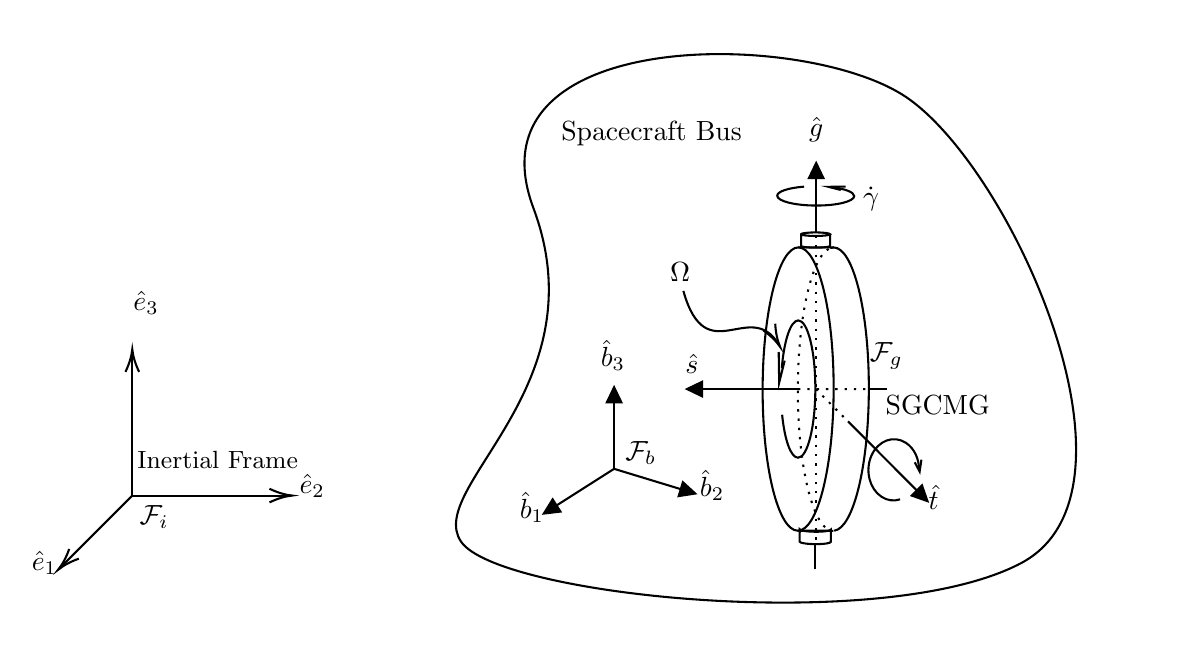
\begin{tikzpicture}[x=0.75pt,y=0.75pt,yscale=-1,xscale=1]
%uncomment if require: \path (0,300); %set diagram left start at 0, and has height of 300

%Straight Lines [id:da892975500466239] 
\draw    (73.1,228.21) -- (38.71,262.6) ;
\draw [shift={(37.3,264.02)}, rotate = 315] [color={rgb, 255:red, 0; green, 0; blue, 0 }  ][line width=0.75]    (10.93,-3.29) .. controls (6.95,-1.4) and (3.31,-0.3) .. (0,0) .. controls (3.31,0.3) and (6.95,1.4) .. (10.93,3.29)   ;
%Straight Lines [id:da5595617967419346] 
\draw    (73.1,228.21) -- (148.13,228.21) ;
\draw [shift={(150.13,228.21)}, rotate = 180] [color={rgb, 255:red, 0; green, 0; blue, 0 }  ][line width=0.75]    (10.93,-3.29) .. controls (6.95,-1.4) and (3.31,-0.3) .. (0,0) .. controls (3.31,0.3) and (6.95,1.4) .. (10.93,3.29)   ;
%Straight Lines [id:da36715700773366944] 
\draw    (73.1,228.21) -- (73.1,159.69) ;
\draw [shift={(73.1,157.69)}, rotate = 450] [color={rgb, 255:red, 0; green, 0; blue, 0 }  ][line width=0.75]    (10.93,-3.29) .. controls (6.95,-1.4) and (3.31,-0.3) .. (0,0) .. controls (3.31,0.3) and (6.95,1.4) .. (10.93,3.29)   ;
%Shape: Ellipse [id:dp29439730581719936] 
\draw   (394.05,108.64) .. controls (384.6,108.62) and (376.88,139.16) .. (376.8,176.85) .. controls (376.72,214.55) and (384.32,245.12) .. (393.76,245.14) .. controls (403.21,245.16) and (410.93,214.62) .. (411.01,176.93) .. controls (411.09,139.23) and (403.5,108.66) .. (394.05,108.64) -- cycle ;
%Shape: Arc [id:dp10136348529454264] 
\draw  [draw opacity=0] (411.29,245.14) .. controls (420.48,243.96) and (427.89,213.89) .. (427.97,176.96) .. controls (428.05,139.27) and (420.45,108.69) .. (411.01,108.67) .. controls (410.47,108.67) and (409.95,108.77) .. (409.43,108.96) -- (410.86,176.93) -- cycle ; \draw   (411.29,245.14) .. controls (420.48,243.96) and (427.89,213.89) .. (427.97,176.96) .. controls (428.05,139.27) and (420.45,108.69) .. (411.01,108.67) .. controls (410.47,108.67) and (409.95,108.77) .. (409.43,108.96) ;
%Shape: Arc [id:dp2890410550496316] 
\draw  [draw opacity=0][dash pattern={on 0.84pt off 2.51pt}] (412.91,109.1) .. controls (412.29,108.82) and (411.65,108.67) .. (411.01,108.67) .. controls (401.56,108.65) and (393.84,139.19) .. (393.76,176.89) .. controls (393.68,213.1) and (400.69,242.74) .. (409.61,245.04) -- (410.86,176.93) -- cycle ; \draw  [dash pattern={on 0.84pt off 2.51pt}] (412.91,109.1) .. controls (412.29,108.82) and (411.65,108.67) .. (411.01,108.67) .. controls (401.56,108.65) and (393.84,139.19) .. (393.76,176.89) .. controls (393.68,213.1) and (400.69,242.74) .. (409.61,245.04) ;
%Straight Lines [id:da4150676998790832] 
\draw    (394.05,108.64) -- (411.15,108.67) ;
%Straight Lines [id:da016544956486795437] 
\draw    (393.76,245.14) -- (410.87,245.18) ;
%Straight Lines [id:da5278828038695935] 
\draw    (342.23,176.89) -- (393.91,176.89) ;
\draw [shift={(339.23,176.89)}, rotate = 0] [fill={rgb, 255:red, 0; green, 0; blue, 0 }  ][line width=0.08]  [draw opacity=0] (8.93,-4.29) -- (0,0) -- (8.93,4.29) -- cycle    ;
%Shape: Arc [id:dp32526133226027953] 
\draw  [draw opacity=0] (386.19,189.27) .. controls (387.4,201.39) and (390.36,209.95) .. (393.84,209.96) .. controls (398.41,209.97) and (402.15,195.17) .. (402.19,176.91) .. controls (402.23,158.65) and (398.55,143.83) .. (393.98,143.82) .. controls (390.27,143.82) and (387.11,153.52) .. (386.02,166.9) -- (393.91,176.89) -- cycle ; \draw   (386.19,189.27) .. controls (387.4,201.39) and (390.36,209.95) .. (393.84,209.96) .. controls (398.41,209.97) and (402.15,195.17) .. (402.19,176.91) .. controls (402.23,158.65) and (398.55,143.83) .. (393.98,143.82) .. controls (390.27,143.82) and (387.11,153.52) .. (386.02,166.9) ;
\draw  [line width=0.75]  (384.54,159.04) -- (384.77,173.79) -- (387.42,163.21) ;
%Straight Lines [id:da9016484611183913] 
\draw  [dash pattern={on 0.84pt off 2.51pt}]  (393.91,176.89) -- (428.05,176.96) ;
%Straight Lines [id:da7421154457848562] 
\draw    (428.05,176.96) -- (436.57,176.96) ;
%Straight Lines [id:da9164158933331166] 
\draw  [dash pattern={on 0.84pt off 2.51pt}]  (402.46,176.91) -- (402.46,251.6) ;
%Straight Lines [id:da22474019923860356] 
\draw    (402.11,263.79) -- (402.11,251.6) ;
%Straight Lines [id:da8613838029876186] 
\draw    (402.6,101.79) -- (402.6,69.84) ;
\draw [shift={(402.6,66.84)}, rotate = 450] [fill={rgb, 255:red, 0; green, 0; blue, 0 }  ][line width=0.08]  [draw opacity=0] (8.93,-4.29) -- (0,0) -- (8.93,4.29) -- cycle    ;
%Straight Lines [id:da16901097367926288] 
\draw  [dash pattern={on 0.84pt off 2.51pt}]  (402.46,103.14) -- (402.46,176.91) ;
%Shape: Arc [id:dp65356329999233] 
\draw  [draw opacity=0] (409.35,79.56) .. controls (416.14,80.28) and (420.92,81.97) .. (420.92,83.92) .. controls (420.9,86.49) and (412.59,88.53) .. (402.36,88.48) .. controls (392.12,88.43) and (383.83,86.31) .. (383.84,83.75) .. controls (383.85,81.67) and (389.3,79.94) .. (396.81,79.38) -- (402.38,83.83) -- cycle ; \draw   (409.35,79.56) .. controls (416.14,80.28) and (420.92,81.97) .. (420.92,83.92) .. controls (420.9,86.49) and (412.59,88.53) .. (402.36,88.48) .. controls (392.12,88.43) and (383.83,86.31) .. (383.84,83.75) .. controls (383.85,81.67) and (389.3,79.94) .. (396.81,79.38) ;
\draw  [line width=0.75]  (416.79,79.38) -- (408.52,79.45) -- (414.44,80.98) ;

%Straight Lines [id:da8822537280465419] 
\draw    (417.93,192.45) -- (454.91,229.58) ;
\draw [shift={(457.03,231.71)}, rotate = 225.12] [fill={rgb, 255:red, 0; green, 0; blue, 0 }  ][line width=0.08]  [draw opacity=0] (8.93,-4.29) -- (0,0) -- (8.93,4.29) -- cycle    ;
%Straight Lines [id:da2857901157034881] 
\draw  [dash pattern={on 0.84pt off 2.51pt}]  (402.46,176.91) -- (417.93,192.45) ;
%Shape: Arc [id:dp592405706333649] 
\draw  [draw opacity=0] (452.15,215.84) .. controls (452.2,210.55) and (449.89,205.42) .. (445.78,202.77) .. controls (439.87,198.95) and (432.47,201.69) .. (429.25,208.89) .. controls (426.04,216.09) and (428.23,225.02) .. (434.14,228.83) .. controls (436.96,230.65) and (440.12,230.98) .. (443,230.04) -- (439.96,215.8) -- cycle ; \draw   (452.15,215.84) .. controls (452.2,210.55) and (449.89,205.42) .. (445.78,202.77) .. controls (439.87,198.95) and (432.47,201.69) .. (429.25,208.89) .. controls (426.04,216.09) and (428.23,225.02) .. (434.14,228.83) .. controls (436.96,230.65) and (440.12,230.98) .. (443,230.04) ;
\draw  [line width=0.75]  (453.3,210.92) -- (452.45,216.64) -- (450.1,212.19) ;
%Curve Lines [id:da7009133041810693] 
\draw    (338.61,129.61) .. controls (349.54,168.5) and (370.6,132.95) .. (384.4,155.15) ;
\draw [shift={(385.23,156.58)}, rotate = 241.27] [color={rgb, 255:red, 0; green, 0; blue, 0 }  ][line width=0.75]    (10.93,-3.29) .. controls (6.95,-1.4) and (3.31,-0.3) .. (0,0) .. controls (3.31,0.3) and (6.95,1.4) .. (10.93,3.29)   ;
%Straight Lines [id:da27425851065851226] 
\draw    (305.24,177.87) -- (305.24,215.33) ;
\draw [shift={(305.24,174.87)}, rotate = 90] [fill={rgb, 255:red, 0; green, 0; blue, 0 }  ][line width=0.08]  [draw opacity=0] (8.93,-4.29) -- (0,0) -- (8.93,4.29) -- cycle    ;
%Straight Lines [id:da26285156144971067] 
\draw    (342.56,226.7) -- (305.24,215.33) ;
\draw [shift={(345.43,227.57)}, rotate = 196.94] [fill={rgb, 255:red, 0; green, 0; blue, 0 }  ][line width=0.08]  [draw opacity=0] (8.93,-4.29) -- (0,0) -- (8.93,4.29) -- cycle    ;
%Straight Lines [id:da04641843522749123] 
\draw    (272.93,235.89) -- (305.24,215.33) ;
\draw [shift={(270.4,237.5)}, rotate = 327.54] [fill={rgb, 255:red, 0; green, 0; blue, 0 }  ][line width=0.08]  [draw opacity=0] (8.93,-4.29) -- (0,0) -- (8.93,4.29) -- cycle    ;
%Shape: Can [id:dp5706734483822697] 
\draw   (409.28,102.29) -- (409.28,107.93) .. controls (409.28,108.4) and (406.16,108.78) .. (402.3,108.78) .. controls (398.44,108.78) and (395.31,108.4) .. (395.31,107.93) -- (395.31,102.29) .. controls (395.31,101.82) and (398.44,101.43) .. (402.3,101.43) .. controls (406.16,101.43) and (409.28,101.82) .. (409.28,102.29) .. controls (409.28,102.76) and (406.16,103.14) .. (402.3,103.14) .. controls (398.44,103.14) and (395.31,102.76) .. (395.31,102.29) ;
%Flowchart: Stored Data [id:dp10460812002274933] 
\draw   (394.62,250.4) -- (394.68,244.43) .. controls (394.67,245.06) and (398.03,245.6) .. (402.17,245.64) .. controls (406.31,245.67) and (409.67,245.19) .. (409.68,244.57) -- (409.63,250.53) .. controls (409.62,251.16) and (406.26,251.64) .. (402.11,251.6) .. controls (397.97,251.57) and (394.62,251.03) .. (394.62,250.4) -- cycle ;

%Shape: Polygon Curved [id:ds2366249191175105] 
\draw   (266.37,89.71) .. controls (234.07,3.28) and (392.09,3.28) .. (443.59,34.71) .. controls (495.1,66.14) and (567.56,225.9) .. (501.21,260.82) .. controls (434.86,295.74) and (248.91,276.53) .. (231.45,250.34) .. controls (213.99,224.15) and (298.67,176.14) .. (266.37,89.71) -- cycle ;

% Text Node
\draw (72.18,128.4) node [anchor=north west][inner sep=0.75pt]    {$\hat{e}_{3}$};
% Text Node
\draw (74.1,205.21) node [anchor=north west][inner sep=0.75pt]  [font=\small] [align=left]  {\small Inertial Frame };
% Text Node
\draw (75.1,231.61) node [anchor=north west][inner sep=0.75pt]    {$\mathcal{F}_{i}$};
% Text Node
\draw (330.73,114.67) node [anchor=north west][inner sep=0.75pt]    {$\Omega $};
% Text Node
\draw (423.69,78.23) node [anchor=north west][inner sep=0.75pt]    {$\dot{\gamma }$};
% Text Node
\draw (455.31,221.77) node [anchor=north west][inner sep=0.75pt]    {$\hat{t}$};
% Text Node
\draw (338.12,158.52) node [anchor=north west][inner sep=0.75pt]    {$\hat{s}$};
% Text Node
\draw (397.65,44.39) node [anchor=north west][inner sep=0.75pt]    {$\hat{g}$};
% Text Node
\draw (426.97,152.93) node [anchor=north west][inner sep=0.75pt]    {$\mathcal{F}_{g}$};
% Text Node
\draw (309.13,200.68) node [anchor=north west][inner sep=0.75pt]    {$\mathcal{F}_{b}$};
% Text Node
\draw (258.3,224.98) node [anchor=north west][inner sep=0.75pt]    {$\hat{b}_{1}$};
% Text Node
\draw (345.11,214.44) node [anchor=north west][inner sep=0.75pt]    {$\hat{b}_{2}$};
% Text Node
\draw (297.36,151.81) node [anchor=north west][inner sep=0.75pt]    {$\hat{b}_{3}$};
% Text Node
\draw (278.28,46.29) node [anchor=north west][inner sep=0.75pt]   [align=left] {Spacecraft Bus};
% Text Node
\draw (434.57,178.5) node [anchor=north west][inner sep=0.75pt]   [align=left] {SGCMG};
% Text Node
\draw (23.2,253.4) node [anchor=north west][inner sep=0.75pt]    {$\hat{e}_{1}$};
% Text Node
\draw (152.18,216.29) node [anchor=north west][inner sep=0.75pt]    {$\hat{e}_{2}$};


\end{tikzpicture}
    \caption{Schematic illustration of Spacecraft with Momentum exchange device}
    \label{fig:tikSGCMGFrame}
\end{figure}

\subsection{Control Moment Gyro Model}
A generic CMG contains a flywheel spinning at constant rate $\displaystyle \Omega $, spin axis is rotated about fixed axis (gimbal axis), this action exerts gyroscopic torque on spacecraft body. Rotation angle $\displaystyle \delta $ is referred as gimbal angle. \autoref{fig:tikCMG} shows generic control moment gyroscope and its axis representation.
\begin{figure}[!ht]
    \centering
    

\tikzset{every picture/.style={line width=0.75pt}} %set default line width to 0.75pt        

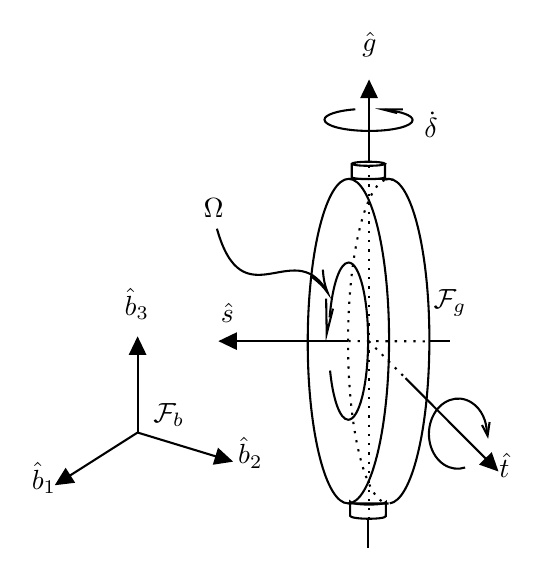
\begin{tikzpicture}[x=0.75pt,y=0.75pt,yscale=-1,xscale=1]
%uncomment if require: \path (0,336); %set diagram left start at 0, and has height of 336

%Shape: Ellipse [id:dp16305937027538286] 
\draw   (198.05,82.18) .. controls (187.23,82.16) and (178.38,117.14) .. (178.29,160.32) .. controls (178.2,203.5) and (186.9,238.52) .. (197.72,238.54) .. controls (208.54,238.57) and (217.39,203.58) .. (217.48,160.4) .. controls (217.57,117.23) and (208.87,82.21) .. (198.05,82.18) -- cycle ;
%Shape: Arc [id:dp5611693860078373] 
\draw  [draw opacity=0] (217.8,238.54) .. controls (228.32,237.19) and (236.81,202.75) .. (236.9,160.44) .. controls (236.99,117.27) and (228.29,82.25) .. (217.47,82.22) .. controls (216.86,82.22) and (216.26,82.33) .. (215.66,82.55) -- (217.31,160.4) -- cycle ; \draw   (217.8,238.54) .. controls (228.32,237.19) and (236.81,202.75) .. (236.9,160.44) .. controls (236.99,117.27) and (228.29,82.25) .. (217.47,82.22) .. controls (216.86,82.22) and (216.26,82.33) .. (215.66,82.55) ;
%Shape: Arc [id:dp4673444196641876] 
\draw  [draw opacity=0][dash pattern={on 0.84pt off 2.51pt}] (219.65,82.71) .. controls (218.94,82.39) and (218.21,82.23) .. (217.47,82.22) .. controls (206.65,82.2) and (197.8,117.19) .. (197.71,160.36) .. controls (197.63,201.84) and (205.65,235.79) .. (215.88,238.42) -- (217.31,160.4) -- cycle ; \draw  [dash pattern={on 0.84pt off 2.51pt}] (219.65,82.71) .. controls (218.94,82.39) and (218.21,82.23) .. (217.47,82.22) .. controls (206.65,82.2) and (197.8,117.19) .. (197.71,160.36) .. controls (197.63,201.84) and (205.65,235.79) .. (215.88,238.42) ;
%Straight Lines [id:da3790853736007833] 
\draw    (198.05,82.18) -- (217.64,82.22) ;
%Straight Lines [id:da49457185352382926] 
\draw    (197.72,238.54) -- (217.31,238.58) ;
%Straight Lines [id:da17676236612848806] 
\draw    (138.25,160.36) -- (197.88,160.36) ;
\draw [shift={(135.25,160.36)}, rotate = 0] [fill={rgb, 255:red, 0; green, 0; blue, 0 }  ][line width=0.08]  [draw opacity=0] (8.93,-4.29) -- (0,0) -- (8.93,4.29) -- cycle    ;
%Shape: Arc [id:dp4399957822164926] 
\draw  [draw opacity=0] (189.05,174.54) .. controls (190.43,188.43) and (193.82,198.23) .. (197.81,198.24) .. controls (203.05,198.25) and (207.33,181.3) .. (207.38,160.38) .. controls (207.42,139.46) and (203.21,122.5) .. (197.96,122.49) .. controls (193.72,122.48) and (190.1,133.59) .. (188.85,148.93) -- (197.88,160.36) -- cycle ; \draw   (189.05,174.54) .. controls (190.43,188.43) and (193.82,198.23) .. (197.81,198.24) .. controls (203.05,198.25) and (207.33,181.3) .. (207.38,160.38) .. controls (207.42,139.46) and (203.21,122.5) .. (197.96,122.49) .. controls (193.72,122.48) and (190.1,133.59) .. (188.85,148.93) ;
\draw  [line width=0.75]  (187.16,139.92) -- (187.42,156.81) -- (190.46,144.7) ;
%Straight Lines [id:da34755210780323087] 
\draw  [dash pattern={on 0.84pt off 2.51pt}]  (197.88,160.36) -- (237,160.45) ;
%Straight Lines [id:da33567491224781065] 
\draw    (237,160.45) -- (246.76,160.45) ;
%Straight Lines [id:da23155226852556665] 
\draw  [dash pattern={on 0.84pt off 2.51pt}]  (207.68,160.38) -- (207.68,245.94) ;
%Straight Lines [id:da35771586989491655] 
\draw    (207.29,259.9) -- (207.29,245.94) ;
%Straight Lines [id:da9106574700939476] 
\draw    (207.84,74.34) -- (207.84,37.31) ;
\draw [shift={(207.84,34.31)}, rotate = 450] [fill={rgb, 255:red, 0; green, 0; blue, 0 }  ][line width=0.08]  [draw opacity=0] (8.93,-4.29) -- (0,0) -- (8.93,4.29) -- cycle    ;
%Straight Lines [id:da20216065712708864] 
\draw  [dash pattern={on 0.84pt off 2.51pt}]  (207.68,75.89) -- (207.68,160.38) ;
%Shape: Arc [id:dp3776892833505412] 
\draw  [draw opacity=0] (215.57,48.87) .. controls (223.35,49.7) and (228.83,51.64) .. (228.82,53.87) .. controls (228.81,56.81) and (219.29,59.15) .. (207.57,59.09) .. controls (195.84,59.04) and (186.35,56.61) .. (186.36,53.67) .. controls (186.37,51.29) and (192.61,49.31) .. (201.21,48.67) -- (207.59,53.77) -- cycle ; \draw   (215.57,48.87) .. controls (223.35,49.7) and (228.83,51.64) .. (228.82,53.87) .. controls (228.81,56.81) and (219.29,59.15) .. (207.57,59.09) .. controls (195.84,59.04) and (186.35,56.61) .. (186.36,53.67) .. controls (186.37,51.29) and (192.61,49.31) .. (201.21,48.67) ;
\draw  [line width=0.75]  (224.09,48.67) -- (214.62,48.75) -- (221.4,50.5) ;

%Straight Lines [id:da42306237074586406] 
\draw    (225.4,178.18) -- (268.07,221.03) ;
\draw [shift={(270.19,223.16)}, rotate = 225.12] [fill={rgb, 255:red, 0; green, 0; blue, 0 }  ][line width=0.08]  [draw opacity=0] (8.93,-4.29) -- (0,0) -- (8.93,4.29) -- cycle    ;
%Straight Lines [id:da4976906999555484] 
\draw  [dash pattern={on 0.84pt off 2.51pt}]  (207.68,160.38) -- (225.4,178.18) ;
%Shape: Arc [id:dp8643023736796815] 
\draw  [draw opacity=0] (264.6,204.98) .. controls (264.66,198.91) and (262.02,193.04) .. (257.3,190) .. controls (250.53,185.63) and (242.05,188.78) .. (238.37,197.02) .. controls (234.69,205.26) and (237.2,215.49) .. (243.97,219.86) .. controls (247.2,221.94) and (250.82,222.32) .. (254.12,221.25) -- (250.64,204.93) -- cycle ; \draw   (264.6,204.98) .. controls (264.66,198.91) and (262.02,193.04) .. (257.3,190) .. controls (250.53,185.63) and (242.05,188.78) .. (238.37,197.02) .. controls (234.69,205.26) and (237.2,215.49) .. (243.97,219.86) .. controls (247.2,221.94) and (250.82,222.32) .. (254.12,221.25) ;
\draw  [line width=0.75]  (265.92,199.34) -- (264.94,205.9) -- (262.25,200.8) ;
%Curve Lines [id:da9723591382724126] 
\draw    (134.54,106.2) .. controls (147.07,150.75) and (171.19,110.03) .. (186.99,135.46) ;
\draw [shift={(187.95,137.1)}, rotate = 241.27] [color={rgb, 255:red, 0; green, 0; blue, 0 }  ][line width=0.75]    (10.93,-3.29) .. controls (6.95,-1.4) and (3.31,-0.3) .. (0,0) .. controls (3.31,0.3) and (6.95,1.4) .. (10.93,3.29)   ;
%Straight Lines [id:da23421207250028164] 
\draw    (96.32,161.05) -- (96.32,204.4) ;
\draw [shift={(96.32,158.05)}, rotate = 90] [fill={rgb, 255:red, 0; green, 0; blue, 0 }  ][line width=0.08]  [draw opacity=0] (8.93,-4.29) -- (0,0) -- (8.93,4.29) -- cycle    ;
%Straight Lines [id:da8003600910266351] 
\draw    (139.48,217.55) -- (96.32,204.4) ;
\draw [shift={(142.35,218.42)}, rotate = 196.94] [fill={rgb, 255:red, 0; green, 0; blue, 0 }  ][line width=0.08]  [draw opacity=0] (8.93,-4.29) -- (0,0) -- (8.93,4.29) -- cycle    ;
%Straight Lines [id:da5231524049233922] 
\draw    (58.94,228.17) -- (96.32,204.4) ;
\draw [shift={(56.41,229.78)}, rotate = 327.54] [fill={rgb, 255:red, 0; green, 0; blue, 0 }  ][line width=0.08]  [draw opacity=0] (8.93,-4.29) -- (0,0) -- (8.93,4.29) -- cycle    ;
%Shape: Can [id:dp3666821815276111] 
\draw   (215.5,74.91) -- (215.5,81.37) .. controls (215.5,81.91) and (211.92,82.35) .. (207.5,82.35) .. controls (203.08,82.35) and (199.5,81.91) .. (199.5,81.37) -- (199.5,74.91) .. controls (199.5,74.37) and (203.08,73.93) .. (207.5,73.93) .. controls (211.92,73.93) and (215.5,74.37) .. (215.5,74.91) .. controls (215.5,75.45) and (211.92,75.89) .. (207.5,75.89) .. controls (203.08,75.89) and (199.5,75.45) .. (199.5,74.91) ;
%Flowchart: Stored Data [id:dp10186943512192137] 
\draw   (198.71,244.56) -- (198.77,237.73) .. controls (198.76,238.45) and (202.6,239.07) .. (207.35,239.11) .. controls (212.09,239.15) and (215.95,238.6) .. (215.95,237.88) -- (215.89,244.72) .. controls (215.88,245.44) and (212.03,245.99) .. (207.29,245.94) .. controls (202.54,245.9) and (198.7,245.28) .. (198.71,244.56) -- cycle ;


% Text Node
\draw (88.61,133.55) node [anchor=north west][inner sep=0.75pt]    {$\hat{b}_{3}$};
% Text Node
\draw (143.3,205.28) node [anchor=north west][inner sep=0.75pt]    {$\hat{b}_{2}$};
% Text Node
\draw (43.86,217.35) node [anchor=north west][inner sep=0.75pt]    {$\hat{b}_{1}$};
% Text Node
\draw (102.38,188.87) node [anchor=north west][inner sep=0.75pt]    {$\mathcal{F}_{b}$};
% Text Node
\draw (237.43,134.17) node [anchor=north west][inner sep=0.75pt]    {$\mathcal{F}_{g}$};
% Text Node
\draw (203.11,9.84) node [anchor=north west][inner sep=0.75pt]    {$\hat{g}$};
% Text Node
\draw (134.93,140.57) node [anchor=north west][inner sep=0.75pt]    {$\hat{s}$};
% Text Node
\draw (269.17,213.02) node [anchor=north west][inner sep=0.75pt]    {$\hat{t}$};
% Text Node
\draw (232.94,48.46) node [anchor=north west][inner sep=0.75pt]    {$\dot{\delta }$};
% Text Node
\draw (126.68,90.2) node [anchor=north west][inner sep=0.75pt]    {$\Omega $};


\end{tikzpicture}

    \caption{Axis definition for generic Control Moment Gyroscope}
    \label{fig:tikCMG}
\end{figure}


Starting from initial gimbal angle $\displaystyle \delta_{0}$ spin and transverse axis as function of $\displaystyle \delta $ are evaluated in $\displaystyle \mathcal{F}_{b}$ as
\begin{equation}
\mathbf{R}( \delta ) =\cos \delta \ \mathbf{1} \ +\ ( 1-\cos \delta ) \ \hat{\mathbf{g}} \otimes \hat{\mathbf{g}} +\sin( \delta ) \ \hat{\mathbf{g}}^{\times }
\end{equation}
\begin{gather}
\hat{s}( t) =\ \mathbf{R}( \delta ) \ \hat{s}( t_{0})\\
\hat{t}( t) =\ \mathbf{R}( \delta ) \ \hat{t}( t_{0}) \notag
\end{gather}
\begin{equation}
\begin{pmatrix}
\hat{s}( t)\\
\hat{t}( t)
\end{pmatrix} =\begin{pmatrix}
\cos( \delta -\delta_{0}) & \sin( \delta -\delta_{0})\\
-\sin( \delta -\delta_{0}) & \cos( \delta -\delta_{0})
\end{pmatrix}\begin{pmatrix}
\hat{s}( t_{0})\\
\hat{t}( t_{0})
\end{pmatrix}
\end{equation}
Angular velocity vector gimbal frame $\displaystyle \mathcal{F}_{g}$ with respect to $\displaystyle \mathcal{F}_{b}$ is 
\begin{equation}
\omega _{\mathcal{F}_{g} /\mathcal{F}_{b}} =\dot{\delta}\hat{g}
\end{equation}
and angular velocity vector of reaction wheel frame $\displaystyle \mathcal{F}_{w}$ in $\displaystyle \mathcal{F}_{g}$ is represented as
\begin{equation}
\omega _{\mathcal{F}_{W} /\mathcal{F}_{g}} =\dot{\delta}\hat{g}
\end{equation}
Gimbal inertia matrix expressed in $\displaystyle \mathcal{F}_{G}$ as diagonal matrix with $\displaystyle J^{*}_{g}$ are gimbal frame inertia along superscript * represented as spin $\displaystyle \hat{s} \ $transverse $\displaystyle \hat{t}$ and $\displaystyle \hat{g}$ axis Subscript $G$ and $W$  $CMG$are used to identify gimbal, RW and CMG respectively.


\begin{gather}
J_{G} =\begin{pmatrix}
J^{s}_{G} & 0 & 0\\
0 & J^{t}_{G} & 0\\
0 & 0 & J^{g}_{G}
\end{pmatrix} \notag
\end{gather}
Flywheel inertia $\displaystyle J^s_{W}$ is much larger than gimbal inertia and is symmetric about $\displaystyle \hat{g}$ therefore $\displaystyle ^{\mathcal{F}_{W}} J_{W} =^{\mathcal{F} g} J_{s}$ thus reaction wheel inertia about spin axis are given by $\displaystyle J^{s}_{W}$ and $\displaystyle J^{t}_{W} =J^{g}_{W}$

\begin{equation}
J_{W} =\begin{pmatrix}
J^{s}_{W} & 0 & 0\\
0 & J^{t}_{W} & 0\\
0 & 0 & J^{t}_{W}
\end{pmatrix}
\end{equation}
Constant diagonal matrix $\displaystyle J_{g}$ and $\displaystyle J_{s}$ are expressed in $\displaystyle \mathcal{F}_{b}$ as
\begin{gather}
J_{G} =J^{s}_{G} \ \hat{s} \ \hat{s}^{T} +J^{t}_{G}\hat{t} \ \hat{t}^{T} +\ J^{g}_{G} \ \hat{g} \ \hat{g}^{T}\\
J_{W} =J^{s}_{W} \ \hat{s} \ \hat{s}^{T} +J^{t}_{W}\hat{t} \ \hat{t}^{T} +\ J^{g}_{W} \ \hat{g} \ \hat{g}^{T} \notag
\end{gather}
and tensor of inertia for CMG system is sum of gimbal and reaction wheel inertia and written in $\displaystyle \mathcal{F}_{b}$ \ as
\begin{equation}
J_{CMG} =J^{s}_{CMG} \ \hat{s} \ \hat{s}^{T} +J^{t}_{CMG}\hat{t} \ \hat{t}^{T} +\ J^{g}_{CMG} \ \hat{g} \ \hat{g}^{T}
\end{equation}
CMG as asymmetric moving masses, note that center of mass of reaction wheel does may have offset from gimbal axis inertia property of spacecraft change with gamble rotation and are function of $\displaystyle \delta ( t)$. Using axis angle rotation matrix $\displaystyle \mathbf{R}( \delta )$
\begin{equation}
J_{CMG}( \delta ) =J^{s}_{CMG} \ \mathbf{R}( \delta )\hat{s}_{0} \ \hat{s}^{T}_{0}\mathbf{R}( \delta )^{T} +J^{t}_{CMG}\mathbf{R}( \delta )\hat{t} \ \hat{t}^{T}\mathbf{R}( \delta )^{T} +\ J^{g}_{CMG} \ \hat{g} \ \hat{g}^{T}
\end{equation}
We can see that $\displaystyle J_{CMG}$ is not constant and in order to realize angular momentum of CMG in body frame we need to evaluate derivative of CMG inertia tensor

\begin{equation}
\begin{aligned}
\dot{J}_{CMG} & =J^{s}_{CMG} \ \left[\dot{\hat{s}} \ \hat{s} +\hat{s} \ \dot{\hat{s}}\right] +J^{t}_{CMG}\left[\dot{\hat{t}} \ \hat{t} +\hat{t} \ \dot{\hat{t}}\right]\\
 & =\dot{\delta}\left( J^{s}_{CMG} -J^{t}_{CMG}\right)[\hat{t} \ \hat{s} +\hat{s} \ \hat{t}]
\end{aligned}
\label{eqn:Jcmg_dot}
\end{equation}

From \autoref{eqn:Jcmg_dot} we can say that derivative of CMG inertia tensor is function of gimbal velocity and difference in moment of inertia about spin and transverse axis. Since these are very small compared and $\displaystyle \dot{J}_{CMG}$ is also very low compared to spacecraft inertia.

We have velocity $\displaystyle \omega $ of spacecraft body frame $\displaystyle \mathcal{F}_{b}$ measured in inertial frame $\displaystyle \mathcal{F}_{i}$ now angular velocity $\displaystyle \omega _{G}$ and $\displaystyle \omega_{w}$of gimbal and flywheel are represented in terms  gimbal angular velocity $\displaystyle \Omega_{G}$ and RW angular velocity $\displaystyle \Omega _{W}$ is


\begin{equation}
\begin{aligned}
\omega _{G} & =\omega +\Omega _{G} =\omega +\dot{\delta}\hat{g}\\
\omega _{W} & =\omega +\Omega _{W} =\omega +\dot{\delta}\hat{g} +\Omega \hat{s}
\end{aligned}
\label{eqn:omega_inG}
\end{equation}

From \autoref{eqn:Jcmg_dot} and \autoref{eqn:omega_inG} Gimbal angular momentum $\displaystyle\mathcal{H}_{G}$, RW angular momentum $\displaystyle \mathcal{H}_{W}$, \ and CMG angular momentum $\displaystyle \mathcal{H}_{CMG}$ \ are evaluated as


\begin{equation}
\begin{aligned}
\mathcal{H}_{G} & =J_{G} \cdotp \omega _{G}\\
 & =\omega +\dot{\delta}\hat{g}\\
 & =J_{G} \cdotp \omega +J^{g}_{G} \ \dot{\delta \ }\hat{g}
\end{aligned}
\end{equation}
RW Momentum,
\begin{equation}
\begin{aligned}
\mathcal{H}_{W} & =J_{W} \cdotp \omega _{W}\\
 & =\omega +\dot{\delta}\hat{g} +\Omega \hat{s}\\
 & =J_{W} \cdotp \omega +J^{g}_{W} \ \dot{\delta} \ \hat{g} +J^s_{W} \ \Omega \hat{s}
\end{aligned}
\end{equation}
CMG Momentum is sum of RW and Gimbal momentum as,
\begin{equation}
\begin{aligned}
\mathcal{H}_{CMG} & =\mathcal{H}_{G} +\mathcal{H}_{W}\\
 & =( J_{G} +J_{W}) \cdotp \omega +\ \left( J^{g}_{G} +J^{g}_{W}\right)\dot{\delta} \ \hat{g} +J_{W} \ \Omega \ \hat{s}\\
 & =J_{CMG}( \delta ) \cdotp \omega +\ J^{g}_{CMG} \ \dot{\delta} \ \hat{g} +J^s_{W} \ \Omega \ \hat{s}
\end{aligned}\\
\label{eqn_Hcmg}
\end{equation}
From \autoref{eqn_Hcmg} we can say that CMG angular momentum is function of body, gimbal, RW angular velocity and gimbal angle $\delta$

\section{Spacecraft Attitude Dynamics}
Rigid body having angular momentum $\displaystyle \mathcal{H}$ with respect to center of mass and applied torque $\displaystyle \mathbf{\tau }$, From newton Euler rigid body dynamics we know that rate of change of angular momentum of body is equal to torque applied to it. Time rate of change of angular momentum in body frame is
\begin{gather}
\frac{d\mathcal{H}}{dt} =\mathbf{\tau }\\
\dot{\mathcal{H}} =\mathbf{\tau } \notag
\end{gather}
Using transport theorem derivative of angular momentum expressed in $\displaystyle \mathcal{F}_{I}$ gives us Newton Euler equation for attitude dynamics.
\begin{equation}
\dot{\mathcal{H}} +\omega \times \mathcal{H} =\tau 
\label{eqn:NewtonEulerB}
\end{equation}

\noindent Assuming the hypothesis of rigid body and neglecting all elastic properties of spacecraft in free falling orbit we can expand the torque $\displaystyle \tau $ as combination of disturbance torque $\displaystyle \tau _{d}$ external environmental torque $\displaystyle \tau _{e}$ and control torque $\displaystyle \mathbf{u}$ thus \autoref{eqn:NewtonEulerB} becomes
\begin{equation}
\dot{\mathcal{H}} +\omega \times \mathcal{H} =\tau _{d} +\tau _{e} +\mathbf{u}
\label{eqn:NewtonEulerI}
\end{equation}
Environmental torques $\displaystyle \tau _{e}$ are the major source of external disturbances that influence dynamics of spacecraft. Gravity gradient torques acting on spacecraft due to variation in gravitational pull acting on distributed mass, they provide small but have significant contribution over the period of time. Due to center of pressure is not coincident with center of mass presence of very small air density at Low Earth Orbit, variation in aerodynamic forces distribution causes couple around center of mass. Magnetic materials and current flowing through electrical systems interacts with earths magnetic field causing contributes to external torque. Solar radiation pressure on spacecraft surface exposed to sun produces torque generally significant amount at Geostationary Orbits. These torques $\displaystyle \tau _{e}$ are known and can be modeled. On the other hand those which are not modeled are disturbance torques $\displaystyle \tau _{d}$ these are due to elastic modes, thruster misalignment, uncertainty in center of gravity and rotating parts.

\noindent The demand control torque $\displaystyle \mathbf{u}$ is provided by actuators such as thrusters, momentum devices, magnetotorquer in order to reorient the spacecraft in desired states or to maintain its attitude based on mission requirements. Following section discuss the modeling of momentum deceives to produce $\displaystyle \mathbf{u}$. Bearing in mind that momentum exchange devices operate on the principle of distributing angular momentum among parts of system keeping total angular momentum conserved as a consequence $\displaystyle \mathbf{u}$ is zero as long as any external saturation system is not present. Other torques $\displaystyle \tau _{e}$ and $\displaystyle \tau _{d}$ are disregarded for preliminary modeling. Accordingly equation becomes
\begin{equation}
\dot{\mathcal{H}} +\omega \times \mathcal{H} = 0
\label{eqn:TorqueFreeEOM}
\end{equation}
For the spacecraft equipped with CMG $\displaystyle \mathcal{H}$ is sum of angular momentum of spacecraft platform $\displaystyle \mathcal{H}_{P}$ and CMG $\displaystyle \mathcal{H}_{CMG}$. Whereas Inertia tensor of platform is
\begin{equation}
J_{P} =J_{P,0} +m\sum ^{n}_{k=1}( ||\vec{\mathbf{d}}_{k} ||\ \vec{\mathbf{1}} -\vec{\mathbf{d}}_{k}\vec{\mathbf{d}}_{k})
\end{equation}
Here, $\displaystyle J_{P,0}$ is inertia of platform without CMG and $\displaystyle m$ is mass of $\displaystyle k^{th}$ CMG whose center of mass is at distance $\displaystyle \vec{\mathbf{d}}_{k}$ from center of mass of entire system. The angular momentum of platform is
\begin{equation}
\mathcal{H}_{P} =J_{P} \cdotp \omega 
\end{equation}

Total system angular momentum of spacecraft equipped \ with $\displaystyle n$ number of SGCMGs is 
\begin{tcolorbox}
\begin{equation}
\begin{aligned}
\mathcal{H} & =\mathcal{H}_{P} +\sum ^{n}_{k=1}\mathcal{H}^{k}_{CMG}\\
 & =J_{P} \cdotp \omega +\sum ^{n}_{k=1}\left( J^{k}_{CMG}( \delta_{k}) \cdotp \omega +\ J^{g}_{CMG} \ \dot{\delta}_{k} \ \hat{g}_{k} +J^{s}_{W} \ \Omega _{k} \ \hat{s}_{k}\right)\\
 & =\left[ J_{P} +\sum ^{n}_{k=1} J^{k}_{CMG}( \delta_{k})\right] \cdotp \omega +\ J^{g}_{CMG} \ \sum ^{n}_{k=1}\dot{\delta}_{k} \ \hat{g}_{k} +J^{s}_{W}\sum ^{n}_{k=1} \ \Omega _{k} \ \hat{s}_{k}
\end{aligned}\\
\label{eqn:H_Total}
\end{equation}
\end{tcolorbox}

Time derivative of \autoref{eqn:H_Total} in platform frame $\mathcal{H}_P$ is expressed as

\begin{equation}
\begin{aligned}
\frac{d\mathcal{H}}{dt} & =\left[ J_{P} +\sum ^{n}_{k=1} J^{k}_{CMG}( \delta_{k})\right] \cdotp \dot{\omega } +\\
 & +\sum ^{n}_{k=1}\dot{J}^{k}_{CMG}( \delta_{k}) \cdotp \omega +\\
 & +\ J^{g}_{CMG}\sum ^{n}_{k=1} \ \ddot{\delta}_{k} \ \hat{g}_{k} +J^{s}_{W}\sum ^{n}_{k=1} \ \dot{\Omega }_{k} \ \hat{s}_{k} +\ J^{s}_{W} \ \sum ^{n}_{k=1} \Omega _{k}\dot{\delta}_{k} \ \hat{t}_{k}
\end{aligned}
\end{equation}Substituting inertia derivative from \autoref{eqn:Jcmg_dot} we have
\begin{equation}
\begin{aligned}
\dot{\mathcal{H}} & =\left[ J_{P} +\sum ^{n}_{k=1} J^{k}_{CMG}( \delta_{k})\right] \cdotp \dot{\omega } +\\
 & +\dot{\delta}\left( J^{s}_{CMG} -J^{t}_{CMG}\right)\sum ^{n}_{k=1}(\hat{t}_{k} \ \hat{s}_{k} +\hat{s}_{k} \ \hat{t}_{k}) \cdotp \omega +\\
 & +\ J^{g}_{CMG} \ \sum ^{n}_{k=1}\ddot{\delta}_{k} \ \hat{g}_{k} +J^{s}_{W}\sum ^{n}_{k=1} \ \dot{\Omega }_{k} \ \hat{s}_{k} +\ J^{s}_{W} \ \sum ^{n}_{k=1} \Omega _{k}\dot{\delta}_{k} \ \hat{t}_{k}
\end{aligned}
\label{eqn:TorqueFreeEOM_H}
\end{equation}
Cross multiplying \autoref{eqn:H_Total} by body angular velocity $\omega$ we get gyroscopic part of Euler attitude equation
\begin{equation}
\begin{aligned}
\omega \times \mathcal{H} & =\omega \times \left[ J_{P} +\sum ^{n}_{k=1} J^{k}_{CMG}( \delta_{k})\right] \cdotp \omega \\
 & +\ J^{g}_{CMG} \ \omega \times \sum ^{n}_{k=1}\dot{\delta}_{k} \ \hat{g}_{k}\\
 & +\ J^{s}_{W} \omega \times \sum ^{n}_{k=1} \ \Omega _{k} \ \hat{s}_{k}
\end{aligned}
\label{eqn:TorqueFreeEOM_xH}
\end{equation}
Substituting \autoref{eqn:TorqueFreeEOM_xH} and \autoref{eqn:TorqueFreeEOM_xH} in to \autoref{eqn:TorqueFreeEOM} we have Generalized attitude dynamics of a rigid satellite equipped with a cluster of $\displaystyle n$ identical single gimbal VSCMGs
%///////////////VSCMG EOM/////////////////////


\begin{tcolorbox}
\begin{equation}
\begin{aligned}
\dot{\mathcal{H}} +\omega \times \mathcal{H} & =
\left[ J_{P} +\sum ^{n}_{k=1} J^{k}_{CMG}( \delta_{k})\right] \cdotp \dot{\omega }+\omega \times \left[ J_{P} +\sum ^{n}_{k=1} J^{k}_{CMG}( \delta_{k})\right] \cdotp \omega \\
 & +\ \dot{\delta}\left( J^{s}_{CMG} -J^{t}_{CMG}\right)\sum ^{n}_{k=1}(\hat{t}_{k} \ \hat{s}_{k} +\hat{s}_{k} \ \hat{t}_{k}) \cdotp \omega \\
 & +\ J^{s}_{W}\sum ^{n}_{k=1} \ \dot{\Omega }_{k} \ \hat{s}_{k} +\ J^{s}_{W} \ \sum ^{n}_{k=1} \Omega _{k}\dot{\delta}_{k} \ \hat{t}_{k} +\ J^{s}_{W} \omega \times \sum ^{n}_{k=1} \ \Omega _{k} \ \hat{s}_{k}\\
 & +J^{g}_{CMG} \ \sum ^{n}_{k=1}\ddot{\delta}_{k} \ \hat{g}_{k} +J^{g}_{CMG} \ \omega \times \sum ^{n}_{k=1}\dot{\delta}_{k} \ \hat{g}_{k}
\end{aligned}
\label{eqn:EOM_FULL}
\end{equation}
\end{tcolorbox}

%//////////////////END EOM/////////////////////
Dynamical equation \autoref{eqn:EOM_FULL} is composition of contribution effects due to spacecraft angular velocity, gyroscopic effects the angular momentum of the entire system, variation of moment of inertia flywheel and gimbal velocities explained in \autoref{tab:vscmg_eom_explain} as reasoning \ of each terms contribution in entire system dynamics.A generalized dynamics for a satellite equipped with generic number of momentum exchange devices. We can see that this equation of motion comprises dynamics of reaction wheel, CMG and VSCMG 
\begin{table}[!ht]
\centering
\begin{tabular}{p{0.30\textwidth}||p{0.7\textwidth}}
\toprule
\begin{center} Contribution rationale  \end{center}& \begin{center}
     Term
 \end{center} \\
\midrule
Variation of satellite angular velocity & 
\begin{equation*}
\left[ J_{P} +\sum ^{n}_{k=1} J^{k}_{CMG}( \delta_{k})\right] \cdotp \dot{\omega }
\vspace{-1em}\end{equation*} \\
\hline 
 Gyroscopic effects due to angular momentum of entire system & 
\begin{equation*}
\omega \times \left[ J_{P} +\sum ^{n}_{k=1} J^{k}_{CMG}( \delta_{k})\right] \cdotp \omega 
\vspace{-1em}\end{equation*} \\
\hline 
 variation of the tensor of inertia & 
\begin{equation*}
\dot{\delta}\left( J^{s}_{CMG} -J^{t}_{CMG}\right)\sum ^{n}_{k=1}(\hat{t}_{k} \ \hat{s}_{k} +\hat{s}_{k} \ \hat{t}_{k}) \cdotp \omega 
\vspace{-1em}\end{equation*} \\
\hline 
variation reaction wheel velocities & 
\begin{equation*}
\ J^{s}_{W}\sum ^{n}_{k=1} \ \dot{\Omega }_{k} \ \hat{s}_{k} +\ J^{s}_{W} \ \sum ^{n}_{k=1} \Omega _{k}\dot{\delta}_{k} \ \hat{t}_{k} +\ J^{s}_{W} \omega \times \sum ^{n}_{k=1} \ \Omega _{k} \ \hat{s}
\vspace{-1em}\end{equation*} \\
\hline 
 variation of gimbals velocities & 
\begin{equation*}
J^{g}_{CMG} \ \sum ^{n}_{k=1}\ddot{\delta}_{k} \ \hat{g}_{k} +J^{g}_{CMG} \ \omega \times \sum ^{n}_{k=1}\dot{\delta}_{k} \ \hat{g}_{k}
\vspace{-1em}\end{equation*} \\
\bottomrule
\end{tabular}
    \caption{Explanation of individual terms in generalize equation of motion for satellite with generic number of VSCMG}
    \label{tab:vscmg_eom_explain}
\end{table}

\subsection{Reaction Wheel (RW)}
If we freeze the gimbal, i.e. $\displaystyle \dot{\delta} =0$ in \autoref{eqn:EOM_FULL}, resultant equation is satellite with reaction wheels simplified as
\begin{equation}
\dot{\mathcal{H}} +\omega \times \mathcal{H} =J \cdotp \dot{\omega } +\omega \times J \cdotp \omega +\ J^{s}_{W}\sum ^{n}_{k=1} \ \dot{\Omega }_{k} \ \hat{s}_{k} +\ J^{s}_{W} \omega \times \sum ^{n}_{k=1} \ \Omega _{k} \ \hat{s}_{k} =0
\end{equation}
here $\displaystyle J=J_{P} +\sum ^{n}_{k=1} J^{k}_{CMG}$ and derivative of $\displaystyle \dot{J}$ is zero. For regulation maneuver which conveys maintain fixed attitude counteracting the external disturbance making body rate $\displaystyle \omega =0$ becomes.
\begin{equation}
J^{s}_{W}\sum ^{n}_{k=1} \ \dot{\Omega }_{k} \ \hat{s}_{k} =\tau _{d}
\end{equation}
Three reaction wheels with their spin axis mutually perpendicular are sufficient to counteract disturbance in any axis as long as saturation (maximum limit of angular momentum) does not occurs. Output torque is torque is proportional to rate of change of RW angular velocity and moment of inertia.

\subsection{Control Moment Gyroscope (CMG)}
Keeping angular velocity of RW \ $\displaystyle \Omega $ constant in \autoref{eqn:EOM_FULL} we get e attitude equation of a satellite equipped with control moment gyros as 
\begin{equation}
\begin{aligned}
\dot{\mathcal{H}} +\omega \times \mathcal{H} & =\left[ J_{P} +\sum ^{n}_{k=1} J^{k}_{CMG}( \delta_{k})\right] \cdotp \dot{\omega } +\omega \times \left[ J_{P} +\sum ^{n}_{k=1} J^{k}_{CMG}( \delta_{k})\right] \cdotp \omega \\
 & +\ \dot{\delta}\left( J^{s}_{CMG} -J^{t}_{CMG}\right)\sum ^{n}_{k=1}(\hat{t}_{k} \ \hat{s}_{k} +\hat{s}_{k} \ \hat{t}_{k}) \cdotp \omega \\
 & +\ J^{s}_{W} \ \sum ^{n}_{k=1} \Omega _{k}\dot{\delta}_{k} \ \hat{t}_{k} +\ J^{s}_{W} \omega \times \sum ^{n}_{k=1} \ \Omega _{k} \ \hat{s}_{k}\\
 & +J^{g}_{CMG} \ \sum ^{n}_{k=1}\ddot{\delta}_{k} \ \hat{g}_{k} +J^{g}_{CMG} \ \omega \times \sum ^{n}_{k=1}\dot{\delta}_{k} \ \hat{g}_{k}
\end{aligned}
\end{equation}


For regulation maneuver disturbance torque can be counteracted as
\begin{equation}
J^{s}_{W} \ \sum ^{n}_{k=1} \Omega _{k}\dot{\delta}_{k} \ \hat{t}_{k} +J^{g}_{CMG} \ \sum ^{n}_{k=1}\ddot{\delta}_{k} \ \hat{g}_{k} =\tau _{d}
\label{eqb:cmg_tau_d}
\end{equation}
Torque produced through CMG is sum of gyroscopic couple due to variation in RW axis variation and acceleration of gimbal frame. Since moment of inertia of CMG and acceleration along gimbal axis is very small \autoref{eqb:cmg_tau_d} is simplified as
\begin{equation}
J^{s}_{W} \ \sum ^{n}_{k=1} \Omega _{k}\dot{\delta}_{k} \ \hat{t}_{k} =\tau _{d}
\label{eqn:cmg_tau}
\end{equation}
\autoref{eqn:cmg_tau} is torque amplification due to gyroscopic effects of RW in body frame which is larger compared to RW. CMG torques are along transverse axis $\displaystyle \hat{t}$ moving in $\displaystyle \mathcal{F}_{b}$ and cannot produce orthogonal torque known as singularity.
\begin{equation}
\begin{aligned}
\dot{\mathcal{H}} +\omega \times \mathcal{H} & =\left[ J_{P} +\sum ^{n}_{k=1} J^{k}_{CMG}( \delta_{k})\right] \cdotp \dot{\omega } +\omega \times \left[ J_{P} +\sum ^{n}_{k=1} J^{k}_{CMG}( \delta_{k})\right] \cdotp \omega \\
 & +\ \dot{\delta}\left( J^{s}_{CMG} -J^{t}_{CMG}\right)\sum ^{n}_{k=1}(\hat{t}_{k} \ \hat{s}_{k} +\hat{s}_{k} \ \hat{t}_{k}) \cdotp \omega \\
 & +\ J^{s}_{W} \ \sum ^{n}_{k=1} \Omega _{k}\dot{\delta}_{k} \ \hat{t}_{k} +\ J^{s}_{W} \omega \times \sum ^{n}_{k=1} \ \Omega _{k} \ \hat{s}_{k}\\
 & +J^{g}_{CMG} \ \sum ^{n}_{k=1}\ddot{\delta}_{k} \ \hat{g}_{k} +J^{g}_{CMG} \ \omega \times \sum ^{n}_{k=1}\dot{\delta}_{k} \ \hat{g}_{k}
\end{aligned}
\end{equation}
For regulation maneuver torque is evaluated as
\begin{equation}
J^{s}_{W} \ \sum ^{n}_{k=1} \Omega _{k}\dot{\delta}_{k} \ \hat{t}_{k} +J^{g}_{CMG} \ \sum ^{n}_{k=1}\ddot{\delta}_{k} \ \hat{g}_{k} =\tau _{d}
\end{equation}
Simplified for small gimbal acceleration, regulation maneuver torque
\begin{equation}
J^{s}_{W} \ \sum ^{n}_{k=1} \Omega _{k}\dot{\delta}_{k} \ \hat{t}_{k} =\tau _{d}
\end{equation}
\subsection{Variable Speed Control Moment Gyroscope (VSCMG)}

Taking advantage from both reaction wheel and CMG for regulation maneuver to neutralize external disturbance $\displaystyle \tau _{d}$ we have
\begin{equation}
\ J^{s}_{W}\sum ^{n}_{k=1} \ \dot{\Omega }_{k} \ \hat{s}_{k} +J^{s}_{W} \ \sum ^{n}_{k=1} \Omega _{k}\dot{\delta}_{k} \ \hat{t}_{k} +J^{g}_{CMG} \ \sum ^{n}_{k=1}\ddot{\delta}_{k} \ \hat{g}_{k} =\tau _{d}
\end{equation}
is combination of RW and torque amplification due to CMG. Trivial presence in CMG can be escaped with RW and high torques are generated with gyroscopic forces. This thesis focuses on VSCMG with pyramid cluster. In order to simplify numerical computation direction vectors can be arranged in matrix form. For n-VSCMG, Unit direction vectors of Gimbal, Spin and Transverse axis axis are evaluated based on their initial orientation

\begin{gather}
\mathcal{G}_{g} =[\hat{g}_{1} \cdots \ \hat{g}_{n}]_{3\times n} =\mathcal{G}_{g_0} \notag\\
\mathcal{G}_{s} \ =\ [\hat{s}_{1} \cdots \ \hat{s}_{n}]_{3\times n} =\mathcal{G}_{s_0}\cos \delta +\mathcal{G}_{t_0}\sin \delta  \notag\\
\mathcal{G}_{t} \ =[\hat{t}_{1} \cdots \ \hat{t}_{n}]_{3\times n} =\mathcal{- G}_{s_0}\sin \delta +\mathcal{G}_{t_0}\cos \delta 
\end{gather}

This thesis is focused on pyramid cluster of four VSCMG units. Single Gimbal Control Moment Gyroscope basis vectors, initially orientation of each CMG spin and gimbal axis is shown in \autoref{fig:VSCMGPyramid} with gimbal axis skewed by angle $\beta$.


\tikzset{every picture/.style={line width=0.75pt}} %set default line width to 0.75pt
\begin{figure}[h]
\centering


\tikzset{every picture/.style={line width=0.75pt}} %set default line width to 0.75pt        

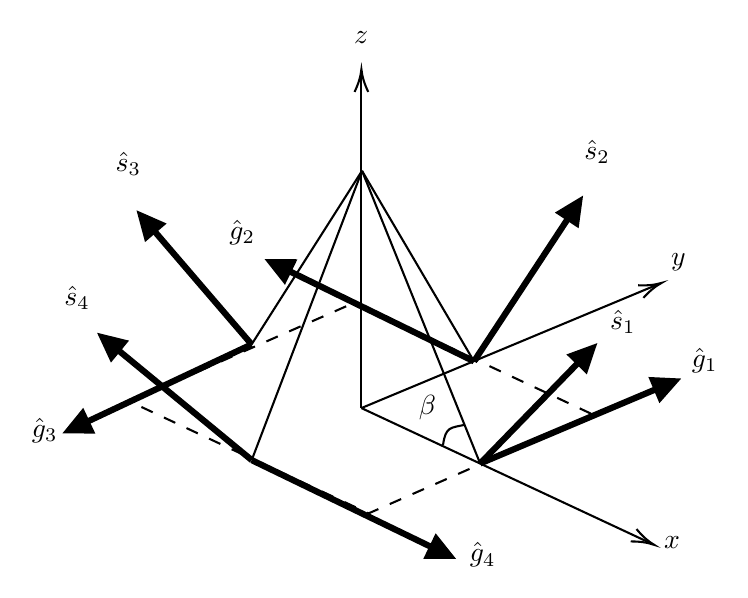
\begin{tikzpicture}[x=0.75pt,y=0.75pt,yscale=-1,xscale=1]
%uncomment if require: \path (0,260); %set diagram left start at 0, and has height of 260

%Shape: Rectangle [id:dp017783013341910126] 
\draw  [dash pattern={on 4.5pt off 4.5pt}] (307.47,113.95) -- (422.51,167.82) -- (314.44,215.41) -- (199.4,161.55) -- cycle ;
%Straight Lines [id:da44988304357834097] 
\draw    (310.95,164.68) -- (450.2,229.75) ;
\draw [shift={(452.01,230.59)}, rotate = 205.05] [color={rgb, 255:red, 0; green, 0; blue, 0 }  ][line width=0.75]    (10.93,-3.29) .. controls (6.95,-1.4) and (3.31,-0.3) .. (0,0) .. controls (3.31,0.3) and (6.95,1.4) .. (10.93,3.29)   ;
%Straight Lines [id:da3169132363517273] 
\draw    (310.95,164.68) -- (310.95,3.43) ;
\draw [shift={(310.95,1.43)}, rotate = 450] [color={rgb, 255:red, 0; green, 0; blue, 0 }  ][line width=0.75]    (10.93,-3.29) .. controls (6.95,-1.4) and (3.31,-0.3) .. (0,0) .. controls (3.31,0.3) and (6.95,1.4) .. (10.93,3.29)   ;
%Straight Lines [id:da03800207830963842] 
\draw [line width=2.25]    (368.16,191.38) -- (460.41,152.4) ;
\draw [shift={(465.02,150.45)}, rotate = 517.0899999999999] [fill={rgb, 255:red, 0; green, 0; blue, 0 }  ][line width=0.08]  [draw opacity=0] (14.29,-6.86) -- (0,0) -- (14.29,6.86) -- cycle    ;
%Straight Lines [id:da7176914327617441] 
\draw    (310.95,164.68) -- (453.78,105.11) ;
\draw [shift={(455.63,104.35)}, rotate = 517.36] [color={rgb, 255:red, 0; green, 0; blue, 0 }  ][line width=0.75]    (10.93,-3.29) .. controls (6.95,-1.4) and (3.31,-0.3) .. (0,0) .. controls (3.31,0.3) and (6.95,1.4) .. (10.93,3.29)   ;
%Straight Lines [id:da7179733571465603] 
\draw [line width=2.25]    (171.44,174.72) -- (258.05,134.01) ;
\draw [shift={(166.92,176.85)}, rotate = 334.82] [fill={rgb, 255:red, 0; green, 0; blue, 0 }  ][line width=0.08]  [draw opacity=0] (14.29,-6.86) -- (0,0) -- (14.29,6.86) -- cycle    ;
%Straight Lines [id:da8667824746636326] 
\draw [line width=2.25]    (258.1,189.75) -- (352.1,235.22) ;
\draw [shift={(356.6,237.4)}, rotate = 205.81] [fill={rgb, 255:red, 0; green, 0; blue, 0 }  ][line width=0.08]  [draw opacity=0] (14.29,-6.86) -- (0,0) -- (14.29,6.86) -- cycle    ;
%Straight Lines [id:da9218968130041245] 
\draw [line width=2.25]    (365.19,142.16) -- (268.78,95.07) ;
\draw [shift={(264.29,92.88)}, rotate = 386.03] [fill={rgb, 255:red, 0; green, 0; blue, 0 }  ][line width=0.08]  [draw opacity=0] (14.29,-6.86) -- (0,0) -- (14.29,6.86) -- cycle    ;
%Straight Lines [id:da6650223825146806] 
\draw [line width=2.25]    (368.16,191.38) -- (421.11,136.98) ;
\draw [shift={(424.6,133.4)}, rotate = 494.23] [fill={rgb, 255:red, 0; green, 0; blue, 0 }  ][line width=0.08]  [draw opacity=0] (14.29,-6.86) -- (0,0) -- (14.29,6.86) -- cycle    ;
%Straight Lines [id:da37227200254977566] 
\draw [line width=2.25]    (365.19,142.16) -- (414.99,66.52) ;
\draw [shift={(417.74,62.34)}, rotate = 483.36] [fill={rgb, 255:red, 0; green, 0; blue, 0 }  ][line width=0.08]  [draw opacity=0] (14.29,-6.86) -- (0,0) -- (14.29,6.86) -- cycle    ;
%Straight Lines [id:da8487690207159158] 
\draw [line width=2.25]    (258.05,134.01) -- (205.86,73.19) ;
\draw [shift={(202.6,69.4)}, rotate = 409.36] [fill={rgb, 255:red, 0; green, 0; blue, 0 }  ][line width=0.08]  [draw opacity=0] (14.29,-6.86) -- (0,0) -- (14.29,6.86) -- cycle    ;
%Straight Lines [id:da10313815978305096] 
\draw [line width=2.25]    (258.1,189.75) -- (187.46,131.58) ;
\draw [shift={(183.6,128.4)}, rotate = 399.47] [fill={rgb, 255:red, 0; green, 0; blue, 0 }  ][line width=0.08]  [draw opacity=0] (14.29,-6.86) -- (0,0) -- (14.29,6.86) -- cycle    ;
%Straight Lines [id:da577231942329048] 
\draw    (311.24,50.38) -- (368.16,191.38) ;
%Straight Lines [id:da021184935151887796] 
\draw    (311.24,50.38) -- (258.1,189.75) ;
%Straight Lines [id:da9892209684505493] 
\draw    (311.24,50.38) -- (258.05,134.01) ;
%Straight Lines [id:da6195700121447263] 
\draw    (311.24,50.38) -- (365.19,142.16) ;
%Curve Lines [id:da0914926090159498] 
\draw    (350.28,182.46) .. controls (351.53,173.5) and (353.86,174.28) .. (360.87,172.72) ;

% Text Node
\draw (468.7,134.14) node [anchor=north west][inner sep=0.75pt]    {$\hat{g}_{1}$};
% Text Node
\draw (245.81,72.81) node [anchor=north west][inner sep=0.75pt]    {$\hat{g}_{2}$};
% Text Node
\draw (361.74,228.05) node [anchor=north west][inner sep=0.75pt]    {$\hat{g}_{4}$};
% Text Node
\draw (150.66,167.97) node [anchor=north west][inner sep=0.75pt]    {$\hat{g}_{3}$};
% Text Node
\draw (429.3,115.9) node [anchor=north west][inner sep=0.75pt]    {$\hat{s}_{1}$};
% Text Node
\draw (416.84,34.11) node [anchor=north west][inner sep=0.75pt]    {$\hat{s}_{2}$};
% Text Node
\draw (191.08,40.08) node [anchor=north west][inner sep=0.75pt]    {$\hat{s}_{3}$};
% Text Node
\draw (166.37,104.54) node [anchor=north west][inner sep=0.75pt]    {$\hat{s}_{4}$};
% Text Node
\draw (337.16,156.94) node [anchor=north west][inner sep=0.75pt]    {$\beta $};
% Text Node
\draw (455.25,225.33) node [anchor=north west][inner sep=0.75pt]    {$x$};
% Text Node
\draw (458.67,88.63) node [anchor=north west][inner sep=0.75pt]    {$y$};
% Text Node
\draw (306,-18.09) node [anchor=north west][inner sep=0.75pt]    {$z$};


\end{tikzpicture}

\caption{VSCMG Pyramid Cluster initial orientation}
\label{fig:VSCMGPyramid}
\end{figure}

Evaluation of commutative gimbal, spin and transverse axis in represented as $\mathcal{G}_g$,$\mathcal{G}_s$ and $\mathcal{G}_t$ respectively about body frame $\mathcal{G}_b$ with basis vector ${b_1,b_2,b_3}$ alinged with ${x,y,x}$. Gimbale axis of all CMGs are oriented by Skew angle $\beta$ is given as
\begin{equation}
\mathcal{G}_g = 
\begin{pmatrix}
 -\sin{}\beta &      0 & \sin{\beta} &       0 \\
       0 & \sin{\beta} &      0 & -\sin{\beta} \\
  \cos{\beta} & \cos{\beta} & \cos{\beta} &  \cos{\beta}
\end{pmatrix}
\end{equation}
\begin{equation}
\mathcal{G}_s =
\begin{pmatrix}
\cos{\beta} \cos{\delta_1} & -\sin{\delta_2} & -\cos{\beta} \cos{\delta_3} &  \sin{\delta_4} \\
-\sin{\delta_1} & -\cos{\beta} \cos{\delta_2} &  \sin{\delta_3} &  \cos{\beta} \cos{\delta_4} \\
\sin{\beta} \cos{\delta_1} &  \sin{\beta} \cos{\delta_2} &  \sin{\beta} \cos{\delta_3} &  \sin{\beta} \cos{\delta_4} 
\end{pmatrix}
\end{equation}
\begin{equation}
\mathcal{G}_t =
\begin{pmatrix}
\cos{\beta} \sin{\delta_1} &         \cos{\delta_2} & -\cos{\beta} \sin{\delta_3} &       -\cos{\delta_4} \\
       \cos{\delta_1} & -\cos{\beta} \sin{\delta_2} &        -\cos{\delta_3} & \cos{\beta} \sin{\delta_4} \\
\sin{\beta} \sin{\delta_1} &  \sin{\beta} \sin{\delta_2} &  \sin{\beta} \sin{\delta_3} & \sin{\beta} \sin{\delta_4}
\end{pmatrix}
\end{equation}

\autoref{eqn:EOM_FULL} can be written in the form of matrix for as 
\begin{tcolorbox}
\begin{equation}
\begin{aligned}
\dot{\mathcal{H}} +\omega \times \mathcal{H} & =J\dot{\omega } +\omega ^{\times }\left( J\omega +\mathcal{G}_{t} J^{g}_{CMG}\dot{\delta } +\mathcal{G}_{s} J^{s}_{W} \Omega \right)\\
 & +\mathcal{G}_{t}[\dot{\delta }]^{d}\left( J^{s}_{CMG} -J^{t}_{CMG}\right)\mathcal{G}^{T}_{s} +\mathcal{G}_{s}[\dot{\delta }]^{d}\left( J^{s}_{CMG} -J^{t}_{CMG}\right)\mathcal{G}^{T}_{t}\\
 & +\mathcal{G}_{t} J^{s}_{W}[ \Omega ]^{d}\dot{\delta } +\mathcal{G}_{s} J^{s}_{W}\dot{\Omega } +\mathcal{G} J^{g}_{CMG}\ddot{\delta }\\
 & =0
\end{aligned}
\end{equation}

\end{tcolorbox}
here cumulative \ moment of inertia including all SGCMG units and platform is denoted as $\displaystyle J$ 
\begin{equation*}
J=J_{P} +\sum ^{n}_{k=1} J^{k}_{CMG}( \gamma _{k})
\end{equation*}
and $\displaystyle [ \Omega ]^{d}$ and $\displaystyle [\dot{\delta }]^{d}$ are diagonal matrices with elements being RW anguler velocities and gimbal velocities.